\section{Casos d'ús}\label{sec:analysis-visualization-use-cases}

Hem definit els següents casos d'ús:

\begin{itemize}
    \item Recurs més accedit durant un període de temps.
    \item Accessos amb el seu contingut alterat.
    \item Condicions d'accés dels accessos a recursos de l'EPSEVG.
\end{itemize}

\subsection{Recurs més accedit durant un període de temps}\label{subsec:most-accessed-resource}

\textbf{Definició}

\begin{itemize}
    \item Donat un període de temps, volem saber quin, o quins recursos són els més accedits.
    \item També volem esbrinar com ha sigut la seva evolució al llarg del temps.
    Es tracta d'un pic puntual que altera les estadístiques, o s'ha mantingut constant?
    \item Quins paràmetres caracteritzen aquests accessos, vora quines hores es produeixen, mitjançant quins mètodes d'\gls{HTTP} es realitzen, quin és el codi de resposta més habitual, quin és el \textit{User Agent} més comú \dots i molts més atributs.
\end{itemize}

\noindent \\
\textbf{Anàlisi}

\begin{itemize}
    \item Per esbrinar quins són els recursos més accedits, treballarem directament sobre la base de dades \textit{InfluxDB}.

    A causa de la gran quantitat de dades que s'han d'analitzar, \textit{Grafana} no podria ser capaç d'afrontar aquesta càrrega computacional.

    \item Per aquest període de temps, consultarem tots els accessos a recursos presents (que ja tenim marcats) i agregarem els seus identificadors.

    En acabar el procés, tindrem un conjunt d'identificadors cadascun amb el seu nombre d'aparicions.
    Ordenarem aquest conjunt i obtindrem els recursos més accedits.
\end{itemize}

\clearpage

\noindent \\
\textbf{Representació}

\begin{itemize}
    \item Per fer la representació de les dades primerament hem d'escollir la tipologia de panells que volem utilitzar.
    Com estem parlant d'un anàlisi al llarg del temps, semblar que una sèrie temporal pot quadrar.

    \item Seleccionarem una gràfica de tipus \texttt{Time Series} i afegirem a la part inferior la següent cerca.
    Concretament, estem cercant a \textit{InfluxDB}:
    \begin{itemize}
        \item Període: desembre del 2023.
        \item Accessos que siguin recursos i el seu \textit{\gls{handle}} (identificador) sigui \texttt{2099.1/18556}, que prèviament haurem determinat.
        \item Comptem cada accés i els agrupem per cada dia.
        \item La cerca que utilitzarem és la següent:
    \end{itemize}
\end{itemize}

\noindent
\begin{verbatim}
from(bucket: "upcommons")
  |> range(start: 2023-12-01T00:00:00Z, stop: 2023-12-31T23:59:59Z)
  |> filter(fn: (r) => r["_measurement"] == "tfg")
  |> filter(fn: (r) => r["_field"] == "recurs")
  |> filter(fn: (r) => r["_value"] == "2099.1/18556")
  |> aggregateWindow(every: 1d, fn: count, createEmpty: false)
  |> yield(name: "count")
\end{verbatim}

\clearpage

\noindent \\
\textbf{Resultat}

\begin{figure}[htbp]
    \centerline{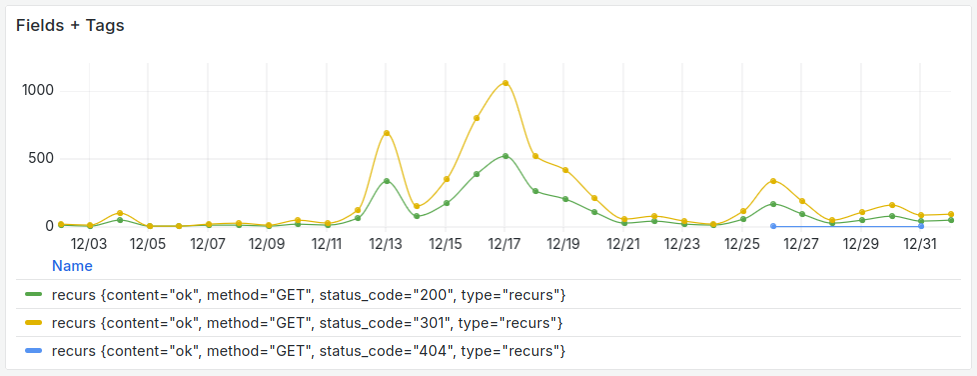
\includegraphics[width=\textwidth]{figures/most-accessed-resource}}
    \captionsetup{justification=centering}
    \caption[Representació del recurs més accedit durant el desembre del 2023.]{Representació del recurs més accedit durant el desembre del 2023. (\textbf{Font}: Elaboració pròpia.)}\label{fig:most-accessed-resource}
\end{figure}

\begin{itemize}
    \item Gràcies al fet que les entrades a la base de dades contenen els camps més rellevants, la classificació per cada paràmetre la realitza \textit{Grafana} automàticament.
    \item Com a conseqüència, per cada combinació del tipus de contingut (\textit{content}), mètode \gls{HTTP} emprat (\textit{method}) i resposta de la petició (\textit{status\_code}) que accedeixin a aquest recurs tindran el seu seguiment.
    \item Podem veure a la llegenda de la figura~\ref{fig:most-accessed-resource}, com sempre el contingut del registre d'accés és correcte (content = “ok”) i el mètode utilitzat és el \texttt{GET}.

    La resposta de la petició varia entre un \texttt{200} (succés) o un \texttt{301} (indica que el contingut és a una altra ubicació i et redirigeix)
\end{itemize}

\clearpage
\subsection{Accessos amb el seu contingut alterat}\label{subsec:content-altered-acces}

\textbf{Definició}

\begin{itemize}
    \item Donat un espai de temps, volem consultar quants accessos s'han produït amb malformacions al seu contingut.

    \begin{itemize}
        \item Les malformacions del contingut del accesos, tal i com vam veure a l'apartat de filtratge dels logs (vegeu filtratge del logs~\ref{subsec:log-filter}), corresponen a registres que difereixen molt respecte el format general.
        \item Durant l'etapa d'anàlisi i emmagatzemmatge dels logs, vam marcar aquells sospitosos amb una etiqueta.
        Concretament, amb content = “diferent”.
    \end{itemize}

    \item També volem esbrinar com ha sigut la seva evolució al llarg del temps, a més dels paràmetres que s'utilitzen.
\end{itemize}

\noindent \\
\textbf{Anàlisi}

\begin{itemize}
    \item Treballarem sobre l'eina d'observabilitat \textit{Grafana}, analitzant aquells accessos a recursos que tinguin alteracions en el seu contingut.
\end{itemize}

\noindent \\
\textbf{Representació}

\begin{itemize}
    \item Per fer la representació de les dades escollirem una sèrie temporal.
    \item Seleccionarem una gràfica de tipus \texttt{Time Series} i afegirem a la part inferior la següent cerca.
    Concretament, estem cercant a \textit{InfluxDB}:

    \begin{itemize}
        \item Període del 2023.
        \item Accessos que siguin recursos i el seu contingut sigui diferent.
        \item Comptem els accessos cada trenta dies.
        \item La cerca que utilitzarem és la següent:
    \end{itemize}
\end{itemize}

\noindent
\begin{verbatim}
from(bucket: "upcommons")
  |> range(start: 2023-01-01T00:00:00Z, stop: 2023-12-31T00:00:00Z)
  |> filter(fn: (r) => r["_measurement"] == "tfg")
  |> filter(fn: (r) => r["_field"] == "log")
  |> filter(fn: (r) => r["type"] == "recurs")
  |> filter(fn: (r) => r["content"] == "diferent")
  |> aggregateWindow(every: 30d, fn: count, createEmpty: false)
  |> yield(name: "count")
\end{verbatim}

\clearpage

\noindent \\
\textbf{Resultat}

\begin{figure}[htbp]
    \centerline{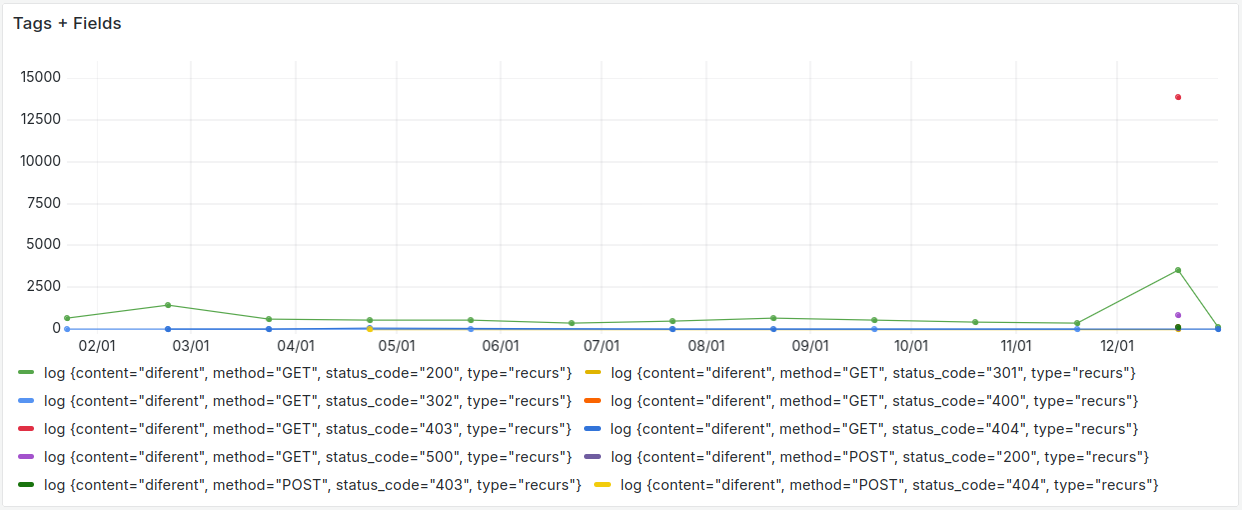
\includegraphics[width=\textwidth]{figures/possible-attacks}}
    \captionsetup{justification=centering}
    \caption[Representació del accessos amb el seu contingut alterat del 2023.]{Representació del accessos amb el seu contingut alterat del 2023. (\textbf{Font}: Elaboració pròpia.)}\label{fig:log-altered}
\end{figure}

\begin{itemize}
    \item Aquest seria el recompte d'accessos a recursos amb el contingut alterat durant l'any 2023, separats per mètode i codi d'estat.
    \item Vora finals d'any (a la part dreta de la figura~\ref{fig:log-altered}), podem observar com hi ha un pic de peticions que no és gens habitual (punt vermell).
    \begin{itemize}
        \item Concretament són peticions \texttt{GET} que retornen un 403.
        \item Conjuntament, hi va haver peticions massives que retornen un codi d'estat correcte, 200.
    \end{itemize}
    \item El codi d'estat 403 del protocol \gls{HTTP} indica que no estas autoritzat per realitzar aquesta petició.
    \item Explorant una mica més, obtenim que aquest pic correspon a una llarga sèrie de peticions que va augmentar considerablement a partir de les 10:30 h de l'11 de novembre del 2023 i hauria acabat quinze minuts després.
    \clearpage
    \begin{figure}[htbp]
        \centerline{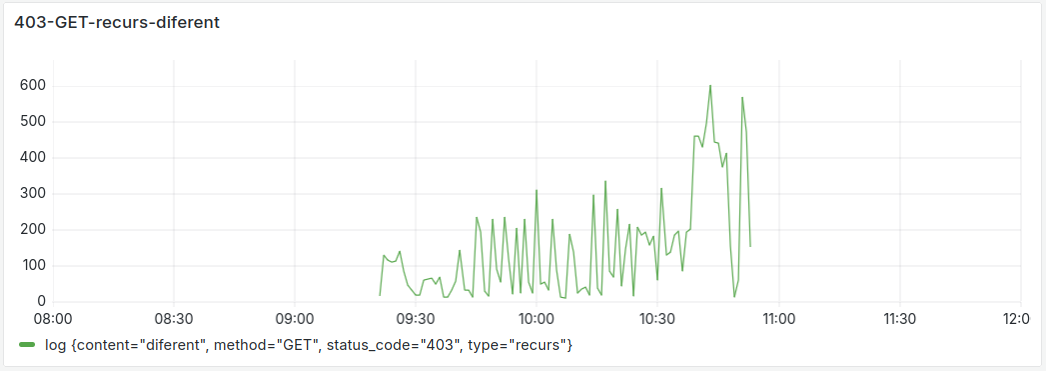
\includegraphics[width=\textwidth]{figures/possible-attacks-403}}
        \captionsetup{justification=centering}
        \caption[Pic de peticions del tipus \texttt{GET} que retornen un codi \texttt{403}.]{Pic de peticions del tipus \texttt{GET} que retornen un codi \texttt{403}. (\textbf{Font}: Elaboració pròpia.)}\label{fig:possible-attacks}
    \end{figure}
    \item Per consultar el contingut d'aquestes peticions ens redirigim a \textit{InfluxDB} i consultem les hores i els paràmetres prèviament determinats.
    \item El diagrama temporal de la figura~\ref{fig:possible-attacks} mostra el següent:
    \begin{itemize}
        \item De les primeres peticions que es van enviar, només unes poques van ser bloquejades, d'aquí ve el màxim de peticions amb un codi 200 de resposta, de la figura~\ref{fig:log-altered}.
        \item Minuts més tard, totes les peticions es van començar a rebutjar.
    \end{itemize}
    \item El patró que segueix és consultar un recurs i afegir paràmetres d'\gls{HTTP} amb valors maliciosos.
    Els més habituals que s'han utilitzat són \texttt{filter} i \texttt{range}.
    La majoria d'aquests registres intenten executar un \texttt{sleep} per endarrerir la resposta certs segons.
    \item Un exemple, la comparació de dues comandes que retornen el mateix resultat sempre és certa (\texttt{now()} i \texttt{sysdate()} a la figura~\ref{fig:log-attack-example}), i s'intenta executar un \texttt{sleep}. \\
    \begin{figure}[htbp]
        \centerline{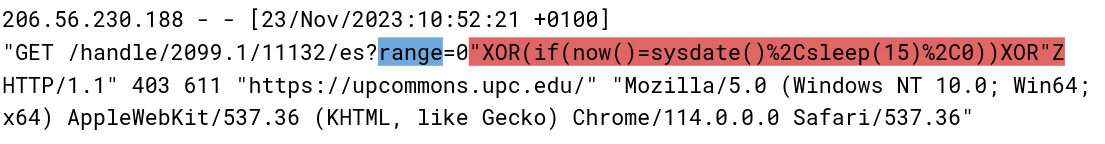
\includegraphics[width=\textwidth]{figures/log-attack}}
        \captionsetup{justification=centering}
        \caption[Exemple d'un intent d'atac a través d'un accés a un recurs.]{Exemple d'un intent d'atac a través d'un accés a un recurs. (\textbf{Font}: UPCommons.)}\label{fig:log-attack-example}
    \end{figure}
\end{itemize}

\clearpage

\subsection{Condicions d'accés dels accessos a recursos de l'EPSEVG}\label{subsec:acces-conditions}

\textbf{Definició}

\begin{itemize}
    \item Donat un període de temps, volem saber quines són les condicions d'accés dels recursos de l'EPSEVG consultats.
    \item Volem analitzar dels registres aquells que siguin accessos a recursos de l'EPSEVG, i determinar si aquests són d'accés obert, restringits per l'usuari, per acord de confidencialitat, restringit a la comunitat universitària, etcètera.
\end{itemize}

\noindent \\
\textbf{Anàlisi}

\begin{itemize}
    \item Per obtenir aquestes dades treballarem tant amb la base de dades dels \textit{\gls{log}s} \textit{InluxDB} com amb les metadades, a \textit{MongoDB}.
    \item Per començar, consultem tots els accessos a recursos durant el període de temps determinat.
    En el nostre cas escollim el dia 2023/12/01.
    \item Per cada accés, consultem la base de dades per obtenir el document de metadades relacionat.
    En cas d'obtenir resultat, consultem l'etiqueta que ens indica el centre docent relacionat amb el recurs: \textit{dc.audience.mediator}.
    \begin{itemize}
        \item Analitzem només aquells que estiguin relacionats amb l'EPSEVG, és a dir, que el contingut de l'etiqueta sigui ``Escola Politècnica Superior d'Enginyeria de Vilanova i la Geltrú''.
    \end{itemize}
    \item Podem obtenir aquest valor pels treballs finals de grau, exàmens, materials docents i vídeos, i d'altres tipologies de manera puntual.
    \item Seguidament, extraiem el valor de l'etiqueta \textit{dc.rights.access}, que conté la informació sobre les condicions d'accés d'aquell recurs.
    \item Agrupant l'identificador del recurs, la condició d'accés i la data i hora de la consulta, afegim aquesta informació a una nova taula a \textit{InfluxDB} anomenada \textit{epsevg-rights}.

\end{itemize}

\clearpage

\noindent \\
\textbf{Representació}

\begin{itemize}
    \item Per fer la representació de les dades escollirem una sèrie temporal.
    \item Seleccionarem una gràfica de tipus \texttt{Time Series} i afegirem a la part inferior la següent cerca.
    Concretament, estem cercant a \textit{InfluxDB}:
    \begin{itemize}
        \item Període del 2023/12/01.
        \item Obtenim tota la informació dels accessos de la taula \textit{epsevg-rights}.
        \item Comptem els accessos cada hora.
        \item La cerca que utilitzarem és la següent:
    \end{itemize}
\end{itemize}

\noindent
\begin{verbatim}
from(bucket: "upcommons")
  |> range(start: 2023-12-01T00:00:00Z, stop: 2023-12-02T00:00:00Z)
  |> filter(fn: (r) => r["_measurement"] == "epsevg-rights")
  |> filter(fn: (r) => r["_field"] == "recurs")
  |> aggregateWindow(every: 1h, fn: count, createEmpty: false)
  |> yield(name: "count")
\end{verbatim}

\clearpage

\noindent \\
\textbf{Resultat}

\begin{figure}[htbp]
    \centerline{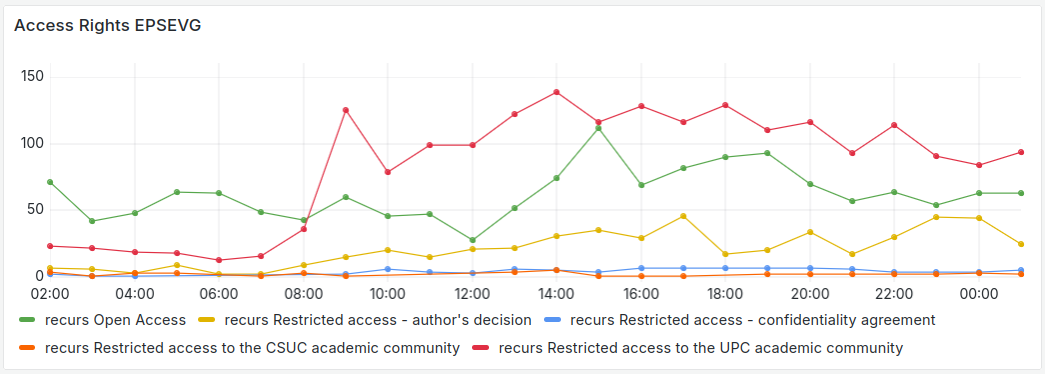
\includegraphics[width=\textwidth]{figures/access-rights-epsevg}}
    \captionsetup{justification=centering}
    \caption[Condicions d'accés dels accessos a recursos de l'EPSEVG el primer de desembre del 2023.]{Condicions d'accés dels accessos a recursos de l'EPSEVG el primer de desembre del 2023. (\textbf{Font}: Elaboració pròpia.)}\label{fig:log-access-type}
\end{figure}

\begin{itemize}
    \item Les diferents condicions d'accés d'aquest període per accessos a recursos, representades a la figura~\ref{fig:log-access-type}, són:
    \begin{itemize}
        \item Vermell: recurs restringit a la comunitat acadèmica de la UPC.
        \item Verd: recurs d'accés obert.
        \item Groc: recurs restringit per decisió de l'autor.
        \item Blau: recurs restringit per acord de confidencialitat
        \item Taronja: recurs restringit a la comunitat acadèmica del CSUC (Consorci de Serveis Universitaris de Catalunya)
    \end{itemize}

    \item Les condicions d'accés més habituals són aquelles on més usuaris poden accedir.
    Aquest són l'accés obert i l'accés restringit a la comunitat acadèmica de la UPC.
    \item Cal remarcar que tots els exàmens són restringits a la comunitat acadèmica de la UPC.
    \item Els menys accedits són aquells d'accés restringit a un públic petit (a vegades nul), sigui per acord de confidencialitat sigui per decisió de l'autor.
    \clearpage
    \item Pel cas dels recursos restringits a la comunitat acadèmica del CSUC (al peu de lletra: “Restricted access to UB, UAB, UPC, UPF, UdG, UdL, URV, UOC, BC, UVic, UJI, URL, UIC users”) es tracta d'accessos a llibres bastant antics.
    \item Dos d'ells tracten principis de desenvolupament sostenible (2099.3/36752 i 2099.3/36834), un altre d'ergonomia (2099.3/36854) i el darrer sobre anàlisi d'antenes (2099.3/36797)

\end{itemize}